%%% LaTeX Template: Article/Thesis/etc. with colored headings and special fonts
%%%
%%% Source: http://www.howtotex.com/
% vim: set spell spelllang=es syntax=tex :

\documentclass[12pt]{article}
\usepackage{styles/apuntes-estilo}
\usepackage{styles/egyptian}
\usepackage{fancyhdr,lastpage}
\usepackage{hyperref}
\usepackage[inline]{enumitem}

\def\maketitle{

\makeatletter
{\color{bl} \centering \huge \sc \textbf{ Trabajo práctico de laboratorio N° 1\\ \large
\vspace*{-8pt} \color{black} Introducción al shell del sistema GNU/LINUX \vspace*{8pt} }\par}
\makeatother

\makeatletter
% vim: set spell spelllang=es syntax=tex :
 {\centering \small 
    Introducción a la computación\\
    Departamento de Ingeniería de Computadoras \\
    Facultad de Informática - Universidad Nacional del Comahue \\
    \vspace{20pt} }
\makeatother

\vspace{-2.5cm}
\mbox{\hspace{-1cm}\includegraphics[width=3cm,height=3cm]{logos/uncoma.pdf}\hspace{12cm}
    
\includegraphics[width=3cm,height=3cm]{logos/fai.pdf}}



}

% Custom headers and footers
\fancyhf{} % clear all header and footer fields
\fancypagestyle{plain}{\fancyhf{}}
\pagestyle{fancy}
\lhead{\footnotesize Laboratorio N° 1 - Introducción al shell del sistema GNU/LINUX}
\rhead{\footnotesize \thepage\ }

\def\ti#1#2{\texttt{#1} & #2 \\ }

\newcommand{\bash}{\textbf{\emph{BASH}}\ }

\begin{document}

\thispagestyle{empty}
\maketitle
\setlength{\parindent}{1pt}

A continuación, se realizarán una serie de ejercicios para los cuales
necesitará acceso a una computadora con el sistema operativo Linux (o una
Máquina Virtual corriendo Linux) y las siguientes aplicaciones:

\begin{itemize}
        
    \item   Intérprete de comandos \bash y demás utilidades que se encuentran
        en la mayoría de las distribuciones de Linux.
        
    \item   Un editor de texto en la interfaz de línea de comando o gráfica.

\end{itemize}

El sistema operativo controla diferentes procesos de una computadora. Uno de
ellos es el intérprete de comandos o \emph{shell}. Este es un programa que
permite al usuario interactuar con el Sistema Operativo. Permite iniciar
(ejecutar) otros programas así como también tiene comandos propios que no
necesitan de otros programas, como por ejemplo comandos para movernos en la
estructura de directorios. En este práctico, utilizaremos el intérprete
\emph{BASH (Bourne-Again SHell)}, muy popular en el mundo de Linux.

Dicho programa debe ser ejecutado en lo que llamamos Terminal o Consola, que
es otro programa que nos permite interactuar mediante el teclado (ingresar
caracteres) y ver los resultados de la ejecución de otros programas en la
pantalla. Al iniciar una consola o terminal de textos, automáticamente se
inicia el \emph{shell} \bash, que es con el que el usuario realmente
interactúa (más abajo se explica esto con un ejemplo).

\section{Sistemas de archivos}

El concepto de directorios (comúnmente llamados ``carpetas'' y archivos es hoy
en día familiar a los usuarios de computadoras, en general el usuario se
maneja visualmente con el ratón y el Explorador de Archivos, utilizando estos
para acceder a los directorios, abrir archivos, ejecutar programas, etc. Podemos
pensar el sistema de archivos como una forma de organizar todo el contenido en
el dispositivo de almacenamiento. Los archivos son datos concretos, utilizan
espacio físico del dispositivo, mientras que las carpetas sirven para
organizar ``lógicamente'' las cosas, igual que una persona tiene estanterías y
cajones en un escritorio para organizar sus papeles.

La figura \ref{arbolDirectorios} muestra un esquema de como se puede pensar en
una estructura de directorios y archivos. \textbf{A}, \textbf{B}, \textbf{C},
\textbf{D}, \textbf{E}, \textbf{G} y \textbf{J} son carpetas o directorios,
\textbf{F}, \textbf{H}, \textbf{I}, \textbf{K}, \textbf{L}, \textbf{M},
\textbf{N} y \textbf{O} son archivos.

\begin{figure}[!htb]

	\centering

	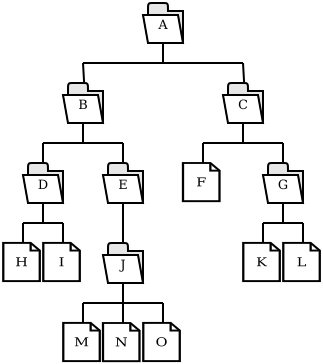
\includegraphics[height=0.45\textheight]{img/directorios.pdf}

	\caption{Árbol de directorios.}

	\label{arbolDirectorios}

\end{figure}

Cuando se inicia el intérprete de comandos, éste se posiciona en una
determinada carpeta, es decir, los comandos que se escriben afectarán
directamente al contenido de dicha carpeta.

En general, al iniciar una consola de texto, junto con un intérprete de
comandos, se posiciona al usuario en la carpeta personal o \textbf{``HOME''}
(en Linux en general es \emph{``/home/usuarioX''}). Desde aquí el usuario
puede navegar por sus archivos y ejecutar comandos.

Además, existen dos formas de hacer referencia a las carpetas y a los archivos
en el intérprete, absoluta y relativa. Cuando utilizamos la forma absoluta se
escribe todo el camino desde la carpeta inicial (en \emph{Linux} se denota con
el símbolo \emph{``/''}) hasta la ubicación deseada. Ejemplos de uso absoluto:
\emph{/home/usuario/trabajo1}, \emph{/etc}, \emph{/tmp}, etc.

El modo relativo sirve para hacer referencia a un directorio que se encuentra
``cerca'' del directorio de trabajo actual en la jerarquía, como por ejemplo
el directorio directamente superior o inferior.

Por ejemplo, las siguientes son direcciones relativas:

\begin{itemize}

    \itemsep2pt \parskip0pt \parsep0pt

    \item \emph{../} (directorio inmediatamente superior)

    \item \emph{./trabajo1} (directorio trabajo1 ubicado dentro del directorio
        actual)

    \item \emph{../../archivoX} (archivo ubicado dos directorios más arriba en
        la jerarquía)

\end{itemize}

\subsection{Entrando en calor con el \emph{shell} \bash}

Inicie el programa mate terminal: \textbf{Aplicaciones → Herramientas del sistema →
Terminal de mate}.

Una vez iniciado, el \emph{shell} \bash en la terminal espera que se escriban
órdenes para ejecutar (comandos). Ejecute y analice cuidadosamente la
siguiente secuencia de comandos en el intérprete \bash (luego de los comandos
y parámetros debe presionar \emph{ENTER}).

Puede consultar el manual de cada uno de los comandos utilizados, usando el
comando \emph{``man nombre\_del\_comando''}, donde se muestran opciones de uso y
se explica la funcionalidad del mismo.

\begin{center}
    \begin{tabular}[t]{|l|l|}
    \hline
        \textbf{Comandos y parámetros} & \textbf{Descripción} \\
    \hline
    \hline
        mkdir e & (crear un directorio de nombre “e”) \\
    \hline
        cd e & (cambiar el directorio actual a “e”) \\
    \hline
        mkdir h1 & (crear un directorio “h1”) \\
    \hline
        mkdir h2 & (crear un directorio “h2”) \\
    \hline
        cd h1 & (cambiar el directorio actual a “h1”) \\
    \hline
        nano a.txt & (crear un archivo de texto y guardarlo) \\
    \hline
        pwd & (imprime el directorio actual) \\
    \hline
        cd .. & (cambiar el directorio actual al directorio padre) \\
    \hline
        pwd & (imprime el directorio actual) \\
    \hline
        cd .. & (cambiar el directorio actual al directorio padre) \\
    \hline
        pwd & (imprime el directorio actual) \\
    \hline
        ls & (listado del directorio actual) \\
    \hline
        ls -R & (listado recursivo de los contenidos) \\
    \hline
        mv e/h1/a.txt e/h2/a.txt & (mueve el archivo a.txt a otro directorio) \\
    \hline
        rm e/h2/ab.txt & (eliminar el archivo ab.txt) \\
    \hline
        rm e/h2/a.txt & (eliminar el archivo a.txt) \\
    \hline
        rmdir e/h1 & (elimina el directorio h1)\\
    \hline
    \end{tabular}

\end{center}

\begin{enumerate}

    \item Realice un esquema visual como el de la figura 1, que muestre la
        estructura de directorios y archivos que se generan hasta el momento
        de la creación del archivo (el comando que usa \emph{``nano''}).

    \item Utilizando los comandos vistos en el listado, reproduzca la
        estructura de directorios y archivos de la Figura 1, respetando
        mayúsculas y nombres de los archivos. Esta estructura será utilizada
        en los subsiguientes incisos.
        
    \item Utilizando la jerarquía de directorios generados en el inciso
        anterior, posicione el intérprete en el directorio A, y realice las
        siguientes acciones:

    \begin{enumerate}

        \item Elimine el archivo ``M'' sin cambiar de directorio.

        \item Mueva los archivos ``H'' e ``I'' a la carpeta ``G''.

        \item Elimine la carpeta ``D''.

        \item Posicione el intérprete en el directorio ``G''.

        \item Sin cambiar de directorio, listar el contenido del directorio
            ``J'' usando directorios relativos.

        \item Sin cambiar de directorio, listar el contenido del directorio
            ``J'' usando directorios absolutos. Para armar una dirección
            absoluta puede usar el comando ``pwd'' para conocer como se
            conforma el camino completo hasta la ubicación actual.

    \end{enumerate}

    \item Explique las ventajas del uso de direcciones ``relativas'' a la
            hora de hacer referencia a otros archivos cercanos en la jerarquía
            al directorio de trabajo actual. Utilice un ejemplo.

    \item Liste el contenido del directorio ``J'', con el comando ``ls -l
        \emph{camino\_a\_J}''.  Analice la información que se muestra por
        pantalla, fecha de creación de los archivos, propietario de los
        archivos y tamaño de los archivos. Modifique alguno de los archivos en
        el editor de texto y vuelva a analizar la salida del comando ``ls
        -l''.

    \item Con el comando ``ls -l'' encuentre un archivo dentro del directorio
        ``/etc'' cuyo tamaño sea mayor a 4KiB, y liste el contenido de dicho
        archivo utilizando los comandos ``cat'', ``more'' y ``less''.

    Teclas útiles:

    \begin{itemize}

        \itemsep2pt \parskip0pt \parsep0pt

        \item cat: no tiene.

        \item more: ``q'' para salir, ``barra espaciadora'' avanzar página.

        \item less: ``q'' para salir, ``barra espaciadora'' avanzar página, y
            ``j'', ''k'' para subir y bajar.

    \end{itemize}

    \item Retorne a su directorio \textbf{HOME}. Para esto ejecute:
        (\textbf{Atención}: el signo \emph{\$} a partir de ahora representa el
        \emph{prompt} del \emph{shell} \bash, no debe escribirlo al ingresar
        cada comando)

        \begin{verbatim}
$ cd           # este es el comando para retornar a su HOME
$ pwd          # pwd le indica cuál es su directorio de trabajo actual
        \end{verbatim}

\end{enumerate}

\subsection{Archivos: nombre, tamaño, tipo, contenido.}

\begin{enumerate}

    \item Asegúrese de que su directorio de trabajo actual es su directorio
        \textbf{HOME} (comando : \emph{pwd}).

    \item Crear un directorio llamado ``misc'' (sin las comillas).

    \item Ingresar al directorio ``misc'' y copiar dentro del mismo los
        siguientes archivos (utilice rutas absolutas con el comando \emph{cp}):

\begin{verbatim}
/etc/passwd
/usr/share/sounds/alsa/Noise.wav
/bin/zcat
/bin/cpio
/usr/share/doc/zenity/NEWS.gz
/usr/share/doc//sudo/README
\end{verbatim}

    \item Una vez copiados, liste los archivos en el directorio misc. Usted
        debería observar que existen seis archivos:

        \begin{verbatim}
$ pwd 
$ ls -l
        \end{verbatim}

    \item El comando ``ls'' anterior le ha entregado información sobre los
        archivos.  Indique el tamaño de cada archivo (en bytes y en KiB).

    \item Observe de qué tipo son los seis archivos en el directorio
        \emph{misc}.  Utilice el comando ``file archivo''. Ejemplo:

        \begin{verbatim}
$ file passwd
        \end{verbatim}

    \item Ahora analizaremos el contenido de cada archivo. Para realizar esta
        tarea obtendremos los primeros 32 bytes de cada archivo. Utilizaremos
        el programa ``hexdump'' para visualizar en base 16 (hexadecimal) el
        valor de cada byte. Ejemplo:

        \begin{verbatim}
$ hexdump -C cpio | head -2
        \end{verbatim}

        El comando anterior le presenta en pantalla el contenido de los
        primeros 32 bytes del archivo \emph{cpio}. Repita la operación para
        cada archivo en el directorio \emph{misc}. Registre los resultados.

    \item Escriba el contenido en base 2 (binario) de los primeros 4 bytes de
        cada archivo.

    \item Sabiendo que cada archivo en el sistema es almacenado en una memoria
        que únicamente puede mantener los datos utilizando componentes
        electrónicos biestables (que mantiene únicamente dos valores
        diferentes) analice y desarrolle un texto que intente explicar cómo es
        posible que los archivos en el sistema sean de diferente ``tipo'' si
        la computadora mantiene únicamente los datos en base 2.

\end{enumerate}

\end{document}
